\documentclass[14pt, a4paper]{extarticle}  % nsk: article -> extarticle
\usepackage[utf8]{inputenc}
\usepackage[T2A,T1]{fontenc}  % nsk

\evensidemargin0cm \oddsidemargin0cm \textwidth16cm
\textheight23cm \topmargin-2cm

% \usepackage[14pt]{extsizes}  % nsk
\usepackage[colorlinks = true,
            linkcolor = blue,
            urlcolor  = blue,
            citecolor = blue,
            unicode,  % nsk
            anchorcolor = blue]{hyperref}

\usepackage[english, ukrainian]{babel}

\usepackage{graphicx}
\usepackage{wrapfig}
\usepackage{lscape}
\usepackage{rotating}
\usepackage{epstopdf}
\usepackage{amsmath}
\usepackage{amsfonts}

\title{Колективний лист від студентів спеціальності ``Прикладна математика''}
% \author{Студенти ОМ-4}
\date{\today}
\begin{document}
\maketitle

%% КОРОЧ. 
%% ТУТ ЩЕ ПРАЦЮВАТИ І ПРАЦЮВАТИ 
Шановні викладачі та адміністрація факультету!

Ми --- студенти факультету комп'ютерних наук та кібернетики, Київського національного університету ім. Тараса Шевченка спеціальності ``прикладна математика''. Впродовж нашого навчання нам неодноразово траплялися курси, лектори та загальні проблеми, які нам би дуже хотілось покращити. Ми щиро розраховуємо в цьому на вашу підтримку. 

Варто зауважити, що цього листа написано винятково через те, що ми б хотіли допомогти поліпшити щось на факультеті, який був для нас другим домом упродовж чотирьох років.

Структура листа буде наступною: спочатку ми сформулюємо головні проблеми, з якими ми зіткнулися, вкажемо на конкретні приклади з пройдених нами курсів, і потім висловимо нашу думку з можливих шляхів покращення. 

\tableofcontents

\newpage
\section{Проблеми:}

\begin{enumerate}
    \item \textbf{Система вибору предметів абсолютно не працює}.
    
    \item \textbf{Застаріла програма} (створена у 70-их роках). Не всі предмети відповідають сучасним вимогам. Деякі спецкурси дуже вузько спрямовані --- що робить їх неактуальними для переважної більшості студентів. У той же час деякі курси не мають достатньо часу, щоб повністю викласти необхідний матеріал. 
    
    Показово, що на спеціальності не читають курсі, що присвячено Python, криптографії, алгоритміці; дослідженню динамічних систем; ; майже нема оптимізації. 
    
    \item  Для багатьох викладачів \textbf{підставою для гарної оцінки є відвідуваність}. Здебільшого це відбувається тоді, коли викладач не може іншими засобами зацікавити студентів до відвідування пар. 
    
    \item Часто викладачі ставлять оцінки, базуючись на суб'єктивному відносному рейтингу студентів у групі. Таким чином гарні оцінки отримують не ті, хто ``знає добре'', а ті, хто ``знає найкраще у групі''.
    
    \item На жаль, трапляється, що викладачі знайомлять студентів не з дисципліною, а зі своїм минулим чи іншими історіями. Безумовно, це важливо, але робити це можна подекуди на перерві при вивченні матеріалу, але аж ніяк не навпаки.
    
    \item Жорстка прив'язка деяких предметів до конкретного програмного забезпечення. Деякі курси вимагають встановлення програм, які коштують як півроку проживання в гуртожитку. Більш того є студенти, які не можуть встановити програму через те, що в них нема OC Windows.
\end{enumerate}

\newpage
\section{Приклади проблем}
\subsection{Другий курс}

\subsubsection{Диференціальні рівняння}

Інколи на практичних заняттях слід розбирати приклади на виведення диференціального рівняння з життєвих задач в областях фізики, хімії, біології, соціології та інших. Це зробило би студентів набагато більш підготовленими до наступних курсів (зокрема, математичної фізики). 

\subsubsection{Комп'ютерна алгебра}

Курс пов'язаний із вивченням ПЗ Maple, що є комерційним, на відміну від ПЗ SageMath, що розробляється за принципами відкритого програмного коду та є абсолютним аналогом Maple. Треба відмітити, що \href{https://webstore.maplesoft.com/catalog.aspx}{Maple Student Edition} коштує 124 \$. Детальніше див. Додаток (\ref{Languages}). 

\subsubsection{Теорія Ймовірностей та Математична статистика}

Зі змінами програми цей предмет перенесено на другий курс, тобто до того як завершиться математичний аналіз. Тому визначення, що пов'язані з теорією міри (сигма-алгебра, інтеграл Лебега) набувають сенсу сильно згодом. Раніше цей курс вивчався на 3-му році бакалаврату, що робило програму більш логічною. 

Наприклад, програма навчання у ХНУ ім. Каразіна така: 
\begin{enumerate}
    \item Математичний аналіз (1--2 курс);
    \item Теорія міри та інтеграл Лебега (5 семестр);
    \item Теорія ймовірностей (6 семестр);
    \item Математична статистика (7 семестр);
    \item Аналіз даних (8 семестр).
\end{enumerate}

\subsubsection{Об'єктно-орієнтоване програмування}
 
Замість цього курсу хотілося б мати курс з ''Алгоритмів та структур даних'', матеріалом якого може стати: як писати різні структури даних (дерева різних типів, хеш-таблиці, тощо); переваги одних над іншими; складність запитів до даних; кількість пам'яті, яку потребує структура даних; різні алгоритми на цих структурах; у яких задачах використовують ці структури або алгоритми.

\subsubsection{Математичний аналіз}

На жаль, курсу не вистачило, щоб розібрати перетворення Фур'є та інтеграл Лебега-Стілтьєса. Ці теми важливі, і на них необхідно виділити додатковий час (можливо за межами курсу). 

\subsubsection{Дослідження операцій}

На практичних заняттях в усіх групах та підгрупах студентам пропонувалось розв'язати рутинні алгоритмічні задачі не на комп'ю\-терах, а на папері. Більш доцільним було б виконання програмованих лабораторних робіт присвячених реалізації вивчених методів. 

Можливо, залучення студентів-старшокурсників допомогло б змінити ситуацію. 

\subsection{Третій курс}
\subsubsection{Аналіз даних}

Через дуже малу кількість практичних занять, основні ідеї та методи курсу залишаються поза увагою студентів. Це є неприпустимим в такому професійно необхідному предметі. З цієї ж причини потік 2019 року випуску не встиг навіть познайомитись з мовою програмування R. Ситуація покращилась у наступних роках та все ж варто звернути увагу на надзвичайну важливість практичних занять в даному курсі. 

\subsubsection{Соціально-політичні студії}
Так як майже кожного року викладачі змінюються, то і система змінюється. 
\begin{itemize}
\item Викладач політології Каращук М. Г.

Дуже проста система оцінювання: законспектувати великий шматок тексту та відвідувати пари. На наступний рік система трохи змінилась: бали були нараховані за результатами контрольних робіт, матеріал яких не викладається на лекціях.

\item Викладачка соціології Тащенко А. Ю. 

Бали нараховуються за презентацію, до якої ніде не прописані вимоги. 
\end{itemize}

\subsubsection{Рівняння математичної фізики}

Правила курсу такі, що оцінювання другого семестру враховує бали за перший: тобто оцінка за перший семестр два рази впливає на середній бал.

\subsubsection{Бази даних та інформаційні системи}
У правилах курсу написано вимоги до лабораторної роботи, які занадто багато уваги приділяють речам, що не пов'язані з предметом курсу (а саме на дизайн  та оформлення), у противагу створенню бази данних чи вмінню нею користуватися. 

Практична частина курсу виконується у СКБД Microsoft Access, хоча зараз існує багато більш популярних і доступних СКБД. Тому можливо було б доцільніше, не прив'язувати суттєву частину курсу до маловживаного ПЗ. Детальніше див. Додаток (\ref{Languages}).

\subsubsection{Теорія прийняття~рішень}
Зміст предмету багато у чому повторює курс ``Дослідження~операцій'', і дуже мало покриває такі теми як прийняття~рішень в умовах~конфлікту ($\approx$ теорія~ігор) та кооперативне прийняття~рішень ($\approx$ теорія кооперативних~ігор). 

Обидва ці підрозділи є  дуже важлививими складовими сучасної~математики (у вже згаданій ВШЕ ``Теорія ігор'' навіть є окремим~\href{https://www.coursera.org/learn/game-theory}{спецкурсом}). 
Викликана така проблема нестачею часу, виділеного на курс.
Мала кількість пар на розгляди нових тем та повна відсутність лабораторних/практичних робіт значно погіршує якість отриманих знань. 

%\subsubsection{Системне програмування}
%Викладач Волохов В.~М. 

%За змістом це доволі гарний курс з дисципліни $\ldots$ ``Побудова компіляторів'' (та синтаксичних і лексичних аналізаторів), але явно не з проектування операційних систем (на що натякає поточна назва). 

%Ба більше, як курс з побудови компіляторів цей курс не є повним. Так, класична книга Ахо і Ульмана ``Компиляторы: принципы, технологии и инструментарий'' (між іншим, доступна у нашій бібліотеці) потребує або одного дуже навантаженого семестру, або цілого року вивчення (у доцільності чого для спеціальності ``прикладна математика'' є певні сумніви). 

%Щоправда, курс (навіть у його поточному змісті) є корисним хоча б тому, що знайомить студентів з рядковими алгоритмами та алгоритмами на графах. Тут ми опускаємо той факт, що це варто було б зробити ще на другому курсі у рамках предмету ``Алгоритми та структури даних.'' 

%Резюмуючи, хотілося б бачити відповідність назви та змісту, причому без втрати поточного змісту у спеціальності загалом, адже він є дуже прикладним і цінним.


\subsubsection{Системне програмування}

За змістом це доволі гарний курс з дисципліни ``Побудова компіляторів'' (та синтаксичних і лексичних аналізаторів), але не з проектування операційних систем (на що натякає поточна назва). 

\subsubsection{Сучасні методи комп'ютерного моделювання}
Один з викладачів Черній Д. І.

Змістовна частина курсу була пов'язана з дослідженням стійкості, що набагато детальніше розібрано в курсі ``Чисельні методи''.

Оцінювання лабораторних робіт не мало чіткої системи і бали студентів були оприлюднені в останній момент. Через те, що  викладач не зміг пояснити як вони були пораховані, склалося враження, що вони ``з'явилися з повітря''. 

\subsection{Четвертий курс}
\subsubsection{Теорія різницевих схем} 
Один з викладачів Черній Д. І.

Курс із теорії різницевих схем мав би містити щось нове відносно того, що було прочитано викладачем у попередньому році на ``Сучасних методах комп'ютерного моделювання'' або до ``Сингулярних задач'', які лектор обіцяв прочитати на магістратурі, або до того, що вже було прочитано на предметі ``Чисельні методи''. 

Кінцеве оцінювання відбувалось просто: всім по 27 з 30 балів. 

\subsubsection{Випадкові процеси}

За відсутності практик предмет є неповноцінним. Через такий суто теоретичний підхід, курс стає схожим на ``довідковий посібник з випадкових процесів''. Наявність практичних занять, домашніх завдань та лабораторних робіт покращило б якість курсу. 

%\subsubsection{Математичне моделювання}
% Викладач Стоян В. А. 
%Курс у тому вигляді, що зараз є, займає набагато більше часу, ніж потрібно. Крім того ідеї курсу, прості для студентів 4-го року навчання, зазвичай складно сприймаються через вкрай незрозумілі формулювання та повну відсутність прикладів. 

%Основна ідея курсу в тому, що розв'язок можна подати у вигляді 
%\begin{align*}
%   y &= y_1 + y_2 + y_3, \\
%   y_1 &= G * u_1, \, y_2 = G * u_2, \, y_3 = G * u_3.
%\end{align*}
%Тут $G(x, y)$ -- функція Гріна для задачі Діріхле. $u_i$ -- спостереження в області та на границі. Але, наприклад, у відомій книзі \href{http://cmcstuff.esyr.org/vmkbotva-r15/4\%20\%D0\%BA\%D1\%83\%D1\%80\%D1\%81/8\%20\%D0\%A1\%D0\%B5\%D0\%BC\%D0\%B5\%D1\%81\%D1\%82\%D1\%80/PDE\%20Extra\%20Chapters\%20\%5BHapaev\%20M.M.\%5D/\%D0\%92.\%D0\%A1.\%20\%D0\%92\%D0\%BB\%D0\%B0\%D0\%B4\%D0\%B8\%D0\%BC\%D0\%B8\%D1\%80\%D0\%BE\%D0\%B2.\%20\%D0\%A3\%D1\%80\%D0\%B0\%D0\%B2\%D0\%BD\%D0\%B5\%D0\%BD\%D0\%B8\%D1\%8F\%20\%D0\%BC\%D0\%B0\%D1\%82\%D0\%B5\%D0\%BC\%D0\%B0\%D1\%82\%D0\%B8\%D1\%87\%D0\%B5\%D1\%81\%D0\%BA\%D0\%BE\%D0\%B9\%20\%D1\%84\%D0\%B8\%D0\%B7\%D0\%B8\%D0\%BA\%D0\%B8.pdf}{``Рівняння математичної фізики'', В.С. Владимирова} у пункті 29.3 для урахування граничних умов використовується похідна функції Гріна, тобто:
%\[ y_2 = \frac{\partial G}{\partial n} * u_2. \]

%В цьому складному моменті викладач, як і всюди, посилається на свої праці або на праці своїх колег по кафедрі. З огляду на це, виникає сумнів у результатах курсу. 

%Просимо звернути увагу, що схожий за назвою курс в КПІ продовжує тематику зовсім інших курсів: ``теорія прийняття рішень'' та ``дослідження операцій''. Чи на ХНУ ім. Каразіна, де предмет викладають на другому курсі, та його тема збігається з темою нашого ``Екологічні і економічні процеси та їх моделювання''. 

\subsubsection{Математичне моделювання}
Курс описує наступну проблему: нехай для диференціального оператора $\mathcal{L}$ відомо функцію Гріна задачі Діріхле $G(t, s)$ та задано рівняння з відомою правою частиною $u$:
\[ \mathcal{L} y = u. \]

Нехай також в деякій області $S$, де діє цей процес, ми фіксуємо спостереження $u^{\partial S}$ на $\partial S$. Якщо б ми мали змогу зафіксувати $u^{\partial S}$ для всіх точок межі області, то задача мала б єдиний розв'язок. Але, якщо наявні лише дискретні спостереження, то основна ідея курсу полягає в тому, що розв'язок можна подати у вигляді:
\begin{align*}
   y &= y^S + y^{\partial S}, \\
   y^S &= G * u, \ y^{\partial S} = G * u^{\partial S}.
\end{align*}

Але, наприклад, у відомій книзі \href{http://cmcstuff.esyr.org/vmkbotva-r15/4\%20\%D0\%BA\%D1\%83\%D1\%80\%D1\%81/8\%20\%D0\%A1\%D0\%B5\%D0\%BC\%D0\%B5\%D1\%81\%D1\%82\%D1\%80/PDE\%20Extra\%20Chapters\%20\%5BHapaev\%20M.M.\%5D/\%D0\%92.\%D0\%A1.\%20\%D0\%92\%D0\%BB\%D0\%B0\%D0\%B4\%D0\%B8\%D0\%BC\%D0\%B8\%D1\%80\%D0\%BE\%D0\%B2.\%20\%D0\%A3\%D1\%80\%D0\%B0\%D0\%B2\%D0\%BD\%D0\%B5\%D0\%BD\%D0\%B8\%D1\%8F\%20\%D0\%BC\%D0\%B0\%D1\%82\%D0\%B5\%D0\%BC\%D0\%B0\%D1\%82\%D0\%B8\%D1\%87\%D0\%B5\%D1\%81\%D0\%BA\%D0\%BE\%D0\%B9\%20\%D1\%84\%D0\%B8\%D0\%B7\%D0\%B8\%D0\%BA\%D0\%B8.pdf}{``Рівняння математичної фізики'', В.С. Владимирова} у пункті 29.3 для урахування граничних умов використовується похідна функції Гріна, тобто:
\[ y^{\partial S} = \frac{\partial G}{\partial n} * u^{\partial S}. \]

В цьому складному моменті викладач, як і всюди, посилається на свої праці або на праці своїх колег по кафедрі. З огляду на це, виникає сумнів у результатах курсу. \medskip

Просимо звернути увагу, що схожий за назвою курс в КПІ продовжує тематику зовсім інших курсів: ``теорія прийняття рішень'' та ``дослідження операцій''. Чи на ХНУ ім. Каразіна, де предмет викладають на другому курсі, та його тема збігається з темою нашого ``Екологічні і економічні процеси та їх моделювання''. В нас було б доцільно читати курс присвячений Машинному навчанню. 

\subsubsection{Прикладні ітераційні методи}
Один з викладачів --- Черній Д. І.

Лабораторна робота повторювала ту, що була запропонована викладачем рік тому на курсі ``Сучасні методи комп'ютерного моделювання''. На першій парі викладач почав розказувати курс ``Інтегральні рівняння'' (зі своїх суб'єктивних міркувань, що, хоча в нашій програмі цього курсу не було, --- він є важливим для магістратури), але загальними поняттями все і завершилось. На подальших заняттях матеріал або повторював те, що було детально розібрано у курсі ``Чисельні методи'', або був присвячиний темі ``Сингулярні задачі''.

\subsection{Спарені предмети}
\label{conjunctions}
На третьому та четвертому курсах нормальної практикою стають спарені предмети: під однією назвою викладаються 2 різні предмети різними викладачами. Здається, вона з'явилась через те, що університет не може створити предмет, що має замалу кількість кредитів. 

Аргументи за розмежування предметів:
\begin{enumerate}
    \item існують предмети, що викладаються та мають малу кількість кредитів (наприклад, 2 кредита мають деякі гуманітарні, 3 --- дискретна математика 2-го семестра). 
    \item цікавий вигляд має оцінювання предметів, що мають дві рівноправні частини, що жодним чином не пов'язані.  
    \item більша кількість предметів --- це краще. Cтудент зможе обирати, що він прослухає; в атестаті залишиться більше відміток.
\end{enumerate}

\subsection{Вибір предметів}
\label{real_choice}
За час нашого навчання нам довелось обирати 7 разів, наприклад, з-поміж ``виборів'' були: % справжні українські реалії
\begin{enumerate}
    \item ``Аналіз стохастичних динамічних систем'' та ``Випадкові процеси''
    \item ``\textbf{Моделі та методи} прийняття рішень'' та ``\textbf{Теорія} прийняття рішень''
    \item  ``Математична логіка та теорія алгоритмів'' та ``Моделі алгоритмів та логічні системи''
    \item ``Архітектура обчислювальних \textbf{машин}'' та ``Архітектура обчислювальних \textbf{систем}''
\end{enumerate}

Складно орієнтуватися на закордонні ВНЗ у цьому питанні, але зверніть увагу на \href{http://appmath.univer.kharkov.ua/courses_new.html}{ХНУ ім. Каразіна}, де дуже багато спецкурсів залишається на вибір студента. 
\newpage

\section{Основні вимоги}
Збільшення кількості студентів упродовж останніх років явно показує, що наш факультет є одним з найперспективніших в Україні для вивчення комп'ютерних наук. Ми щиро сподіваємось, що це також мотивуватиме викладачів винятково до поліпшення якості викладання, а не до повторення помилок, що тягнуться з року в рік. 

Враховуючи все вище сказане, ми наполягаємо на наступних змінах:
\begin{enumerate}
    \item  
    Зрозуміло, що головним фактором рівня освіти є рівень викладання. Студентам важко вказувати викладачам на їхні недоліки. Проте, \textbf{ введення анонімної системи оцінювання навчальних курсів та викладачів} змогло б допомогти їм поліпшити свою роботу. 
    
    \item  \textbf{Зміна системи нарахування балів та вимог до викладання предмету.}
    
    Обов'язкова \textbf{вимога до викладачів чітко називати систему оцінювання та інформувати студентів про свій предмет} на початку семестру: про що йтиметься в курсі; який його зв'язок з іншими предметами; яка його практична цінність; які наукові або практичні досягнення відбулись в останні роки.
    
    Бали необхідно нараховувати \textbf{об'єктивно, а не рейтингово}.
    
    \textbf{Відмова від балів що додаються/знімаються за відвідування}. Не можна оцінити знання за присутністю студента на парі. Для цього існують екзамени та модульні контрольні роботи.
    
    \item \textbf{Реальна, а не фіктивна можливість обирати.} 
    
    Головним важелем у навчанні є бажання студента вивчати предмети, що викладаються. Цікаві та корисні студентам курси залишаються поза увагою лише тому, що вони проводяться на іншій кафедрі чи іншим викладачем в іншій підгрупі. На базі нашого факультету можна частково або повністю \textbf{розмежувати спеціалізації, кафедри та групи}, що реалізувало б можливість для студентів обирати ті курси, що їм до вподоби. Детальніше про це див. (\ref{cathedra_demarcation}). 
\end{enumerate}

\newpage
\section{Шляхи покращення}

Хоч наступні ідеї і потребують часу та зусиль, вони могли б напряму допомогти  вирішити вказані вище проблем. Такі зміни є надзвичайно важливими в переведенні нашого факультету на найкращий навчальний рівень.

\begin{itemize}
    \item  \textbf{Корегування системи курсів разом з  запрошеними спеціалістами} поліпшило б перспективність навчання. Наприклад, представники IT компаній могли б авторитетно підказати які знання вони очікують від майбутніх співробітників і це допомогло б і осучаснити програму, і зробити роботу факультету більш кар'єроспрямо\-ваною.
    
    \item За прикладом багатьох успішних світових ВНЗ на базі чотирьох зв'язаних корпусів --- математики, кібернетики, радіофізики та фізики, --- можна створити систему, де студент обирає предмет та викладача з тих, що наявні на факультетах. Детальніше див. Додаток (\ref{common_space}).
    
    \item  \textbf{Оприлюднювати лекції} в електронному форматі на сайті факультету.
     \textbf{Оприлюднювати завдання} самостійних, модульних, практичних, лабораторних, екзаменаційних, взагалі усіх завдань, що виконуються на факультеті. А також, по можливості, розв'язків до них. Це б і покращило рівень підготовки студентів, і зробило б систему освіти більш прозорою. 
    
    \item \textbf{Перехід на вільне програмне забезпечення}, чи хоча б безкоштовне.
    
    \item В систему навчання було б корисним і цікавим \textbf{вводити онлайн-курси}, що стають дедалі популярнішими. Детальніше див. Додаток (\ref{Additional materials}).
    
    \item Як рішення проблеми спарених предметів можна запропонувати
    \begin{itemize}
        \item називати предмети повними назвами;
        \item проводити їх у дві частини --- тобто першу частину семестра перший предмет, другу --- другий.
    \end{itemize}
    
    \item 
\end{itemize}

\newpage
\section{Щира подяка!}
Нам дуже приємно, що на нашому факультеті є багато ініціатив, чудово побудованих курсів та талановитих викладачів, що абсолютно кваліфіковані у своєму предметі і майстерно виконують свої обов'язки. \textbf{Ми надзвичайно це цінуємо і хотіли б щиро подякувати їм та факультету! }\medskip

Розуміючи, що не можна покращити якість навчання на факультеті, не підтримуючи те, що вже є успішним, нам хотілось би в цьому листі також особливо  відзначити позитивні моменти:
\begin{itemize}
    \item Перш за все таких викладачів як: Номіровський Д. А., Денисов С. В., Семенов В. В., Якимів Р. Я., Карнаух Т. О., Кулян В. Р., Риженко А. І., --- вони професійно вели свої предмети, відповідали на уточнюючі запитання, намагались якнайчіткіше пояснити матеріал і сприяли зацікавленню студентів. 

\item Шарапову М. М.  ми хотіли подякувати за ретельно оформленні матеріали занятть, домашні роботи та чудовий сайт. 

\item Ми також вдячні Пічкуру В. В. за відкритість у прислуханні до критики.

\item Важливо відзначити і деякі факультативи, що запускались під час навчання: ``Deep learning'' від В. В. Дудара; лекції з Алгоритмів від ініціативних студентів. Ми були б раді, якби збільшення їх кількості заохочувалась університетом, або вони і замінили застарілі предмети.

\item Гарною ідеєю є також укладання угод із компаніями, які надають місця для стажувань, наприклад Samsung. Ми були б раді збільшенню кількості таких контрактів.

\item Продовжуючи попередній пункт, ми особливо вдячні за співпрацю з IT-компаніями та проведення фестивалю TetriX. 
\end{itemize}

\newpage
Підписанти:

\begin{tabular}{c|c}
\hline
тут могло би стояти & ваше ім'я \\
\end{tabular}


\newpage\section{Додаток}

\subsection{Онлайн навчання та додаткові матеріали}
\label{Additional materials}
На сьогоднішій день у всьому світі відбувається зміщення фокусу освітніх програм на дистанційне навчання. Наприклад, \href{https://www.hse.ru/ba/am/courses/219906616.html}{курс з Машинного навчання} у ВШЕ, який зараховує проходження онлайн курсу від Стенфордського університету (про який йтиметься далі) як 3 кредита.

Подібні запозичення курсів від найпровідніших університетів світу є дуже малозатратними з точки зору ресурів університету: немає необхідності локалізувати запозичений курс: читати очні лекції, проводити практичні заняття (спільнота слухачів онлайн-курсу набагато більша аніж одна уіверситетська група, і там завжди знайдуться більш досвідчені студенти-модератори які з радістю допоможуть початківцям); онлайн курси мають свою вбудовану систему оцінювання. Єдине, що справді \textbf{потрібне від університету --- бажання і заохочення студентів}.

Також зазначимо, що використання онлайн-курсів дозволяє не просто покращити якість викладання і зробити найкращих викладачів доступними усім студентам, а й реалізувати справжній, а не фіктивний, вибір дисциплін: такі дисципліни можуть входити у програму як зовнішні онлайн-курси, не потребуючи часу викладачів та аудиторій. 

Наведемо тут (на жаль неповний) список курсів, які ми вважаємо релевантним до нашої спеціальності. Зауважимо, що кожен з цих курсів повністю пройдений на гарну оцінку хоча б одним із нас, чим ми підтверджуємо його цілковиту посильність та незаперечну корисність для майбутніх студентів нашої спеціальності:
\begin{enumerate}
    \item \href{https://prometheus.org.ua/entrepreneurship/}{Курс про підприємництво [prometheus]} або \\ \href{https://edx.prometheus.org.ua/courses/NaUKMA/103/2015_T1/about}{Економіка для всіх [prometheus]}.
    
    Зараз на 4-му курсі читають трудове право та підприємництво. Це можна спростити до вимоги пройти один з курсів в спеціалізації.
    
    \item \href{https://www.coursera.org/learn/machine-learning}{Машинне навчання [coursera].}
    
    Вже згаданий курс про машинне навчання від Стенфорда є гарним пунктом будь-якого резюме. При цьому проходження цього курсу не потребує серйозних попередніх знань, окрім, хіба що, математичного аналізу, тобто не є проблемою для студентів факультету кібернетики.
    
    \item \href{https://www.coursera.org/learn/crypto}{Криптографія [coursera].}
    
    Важливий курс для напрямку прикладна математика, якого нажаль взагалі нема в програмі.
    
    \item Серія курсів з математичного аналізу від університету Пенсильванії:
	\begin{enumerate}
		\item \href{https://www.coursera.org/learn/single-variable-calculus/home/welcome}{Вступ до аналізу [coursera].}
		\item \href{https://www.coursera.org/learn/differentiation-calculus/home/welcome}{Диференціювання [coursera].}
		\item \href{https://www.coursera.org/learn/integration-calculus/home/welcome}{Інтегрування [coursera].}
		\item \href{https://www.coursera.org/learn/applications-calculus/home/welcome}{Застосування аналізу [coursera].}
	\end{enumerate}
    
    Курси мають схожу програму з нашими, але при цьому фокус саме на практиці, а не теорії: надзвичайно велика кількість інтерактивних вправ. При цьому професор, що читає лекції часто пропонує альтернативний підхід до найскладніших практичних аспектів математичного аналізу, що значно покращує усвідомлення студетнами матеріалу.

    \item Серія курсів з програмування на C++ від Яндексу:
    \begin{enumerate}
    	\item \href{https://www.coursera.org/learn/c-plus-plus-white/home/welcome}{C++ білий [coursera].}
    	\item \href{https://www.coursera.org/learn/c-plus-plus-yellow/home/welcome}{C++ жовтий [coursera].}
    	\item \href{https://www.coursera.org/learn/c-plus-plus-red/home/welcome}{C++ червоний [coursera].}
    	\item \href{https://www.coursera.org/learn/c-plus-plus-brown/home/welcome}{C++ коричневий [coursera].}
    \end{enumerate}
    Ці курси використовують останній стандарт C++17; вони повністю покривають і, при цьому, суттєво доповнюють програму відповідного курсу, що читається на першому році. Як і у попередній серії, фокус зміщений на практику.

    \item \href{https://www.coursera.org/learn/python-osnovy-programmirovaniya/home/welcome}{Основи програмування на python від Вищої Школи Економіки [coursera]} 
    
    Цей курс представляє щось, чого на нашому факультеті, на превеликий жаль, взагалі немає. При цьому викладається він зрозумілою для усіх наших студентів мовою, і для його інтеграції взагалі нічого не потрібно роботи, окрім проведення очних істипів за відповідними задачами курсу.

    \item Серія спільних курсів про алгоритми та структури даних від університету Каліфорнії, що у Сан Дієго та Вищої Школи Економіки:
    \begin{enumerate}
    	\item \href{https://www.coursera.org/learn/algorithmic-toolbox}{Базові алгоритми [coursera].}
    	\item \href{https://www.coursera.org/learn/data-structures}{Структури даних [coursera].}
    	\item \href{https://www.coursera.org/learn/algorithms-on-graphs}{Алгоритми на графах [coursera].}
    	\item \href{https://www.coursera.org/learn/algorithms-on-strings}{Рядкові алгоритми [coursera].}
    	\item \href{https://www.coursera.org/learn/advanced-algorithms-and-complexity}{Алгоритми та складність [coursera].}
    \end{enumerate}
    Ці курси слугують чудовим прикладом того, як могли б виглядати окремі частини (або навіть увесь курс) алгоритмів на нашому факультеті. 
  
    \item Серія курсів з диференціальних рівнянь від Массачусетського технологічного інституту:
    \begin{enumerate}
    	\item \href{https://www.edx.org/course/introduction-differential-equations-mitx-18-031x}{Рівняння з однією змінною порядку [edx].}
    	\item \href{https://www.edx.org/course/differential-equations-2x2-systems-mitx-18-032x}{Системи рівнянь на площині та математичне моделювання [edx].}
    	\item \href{https://www.edx.org/course/differential-equations-linear-algebra-and-nxn-systems-of-differential-equations}{Загальні системи [edx].}
    	\item \href{https://www.edx.org/course/differential-equations-fourier-series-and-partial-differential-equations}{Рівняння у частинних похідних та аналіз Фур'є [edx].}
    \end{enumerate}
    Ця серія курсів поєднує у собі наші ``Диференціальні рівняння'' та ``Математичне моделювання економічни та екологічних процесів''.

    \item Два курси від МІТ щодо програмування на python:
    \begin{enumerate}
    	\item \href{https://www.edx.org/course/introduction-to-computer-science-and-programming-using-python-0}{Мова програмування python [edx].}
    	\item \href{https://www.edx.org/course/introduction-computational-thinking-data-mitx-6-00-2x-7}{Алгоритми і структури даних у мові python [edx].}
    \end{enumerate}
    Багато у чому схожі на відповідний курс ВШЕ, але при цьому суттєво глибші.

    \item Серія спільних курсів про математичні пререквізити для успішної кар'єри у програмуванні від університету Каліфорнії у Сан Дієго та Вищої Школи Економіки:
    \begin{enumerate}
    	\item \href{https://www.coursera.org/learn/combinatorics}{ Комбінаторика та теорія ймовірності [coursera].}
    	\item \href{https://www.coursera.org/learn/graphs}{Теорія графів [coursera].}
    	\item \href{https://www.coursera.org/learn/number-theory-cryptography}{Теорія чисел і криптографія [coursera].}
    	\item \href{https://www.coursera.org/learn/delivery-problem}{Елементи дослідження операцій [coursera].}
    \end{enumerate}
\end{enumerate}


\subsection{Вивчення та викладання різних мов програмування}
\label{Languages}

Наразі ми вивчаємо C++, далі Maple, далі Java та SQL/Access. 
\begin{itemize}
    \item [Maple.] Mathematica, Maple та SageMath відносятся до класу програм для ``символічних обчислень'', систем комп'ютерної алгебри. Існує й інший набір програм --- так звані ``обчислювальні системи'': Matlab, Octave (його відкритий аналог) та навіть Python, --- вони є більш вживаними. Наприклад, ми неоднаразово помічали стажування (наприклад Mitacs globalink research internship, research internships at IST Austria), де плюсом є їх знання. Курс ``Обробка та розпізнавання зображень'', що вивчається на 4-му році, спирається на знання студента в Matlab/Octave. 
    
    \item [Java.] Вивчається на предметі (Системне програмування), що не мав би концентрувати свою увагу на вивченні саме Java. Нема сенсу прив'я\-зувати предмет до конкретної мови; більш того, коли до цього 2 роки вивчали іншу мову (C++).  
    
    \item [SQL/Access.] Для роботи з базами данних використовується середовище Microsoft Access. \href{https://products.office.com/uk-UA/buy/office}{Річна підписка} на цю ПЗ коштує від 1900 грн. Замість неї можна залишати вибір середовища на розсуд студента. На сьогодні є сенс вивчати більш популярні системи: \textit{postgresql}, \textit{mongodb} або \textit{Hbase}. Усі вони відкриті та безкоштовні. 
\end{itemize}


%(вставить часть про Хаскель)

Враховуючи це, можна сказати, що на другому курсі є сенс запропонувати студентам вибір між різними мовами програмування: Python3, Octave, Sage. 
% До програми додати виборним спецкурсом Haskell.
На базах данних мати більше свободи у практичній частині. 

\subsection{Про розмежування кафедр та груп}
\label{cathedra_demarcation}
Засобом, щоб покращити ситуацію з вибором предметів вбачається розмежування кафедр та груп. Це означає, що після другого курсу групи не формуються стандартним шляхом, а, замість цього, будується розклад, де наявні усі спецкурси, що зазвичай читаються на кафедрах. Далі студенти обирають, які спецкурси вони бажають відвідувати.

Такий підхід до роботи кафедр є логічним, оскільки зараз зазвичай група, а з нею і кафедра, обирається не за можливими науковими інтересами студента, а за принципом ``куди друзі --- туди і я''. Це також змусить викладача організовувати гарний курс, щоб мати попит з боку студентів. Таким чином можна суттєво збільшити кількість виборних предметів, а також відсіяти ті спецкурси, що є нецікавими або неякісними.

Рахуючи спарені предмети як два, на ОМ загалом маємо близько 15-ти предметів. Також під 

\subsection{Про єдиний університетський простір}
\label{common_space}
Корпуси, що знаходяться на ВДНГ, концентрують майже усі технічні спеціальності у КНУ. Це сумно, що досі ми не маємо можливості відвідувати лекції на суміжних факультетах. 

Наше бачення того як це могло би бути таке:
\begin{itemize}
    \item [гуманітарні.] всім на факультеті не подобаються гуманітарні предмети. Це як аксіома. Але, може, збільшення їх розмаїття гарно вплине. Зробити це можна зробити так: на всіх чотирьох корпусах в однаковий час (наприклад, третя пара у п'ятницю) проводити курси з різних гуманітарних предметів. Студенти зможуть записатися на той, що їм більш до вподоби. 
    \item [точні.] так як цих предметів забагато, то їх можна розкидати випадково. Ймовірність, що всім не сподобається досить мала. :) 
\end{itemize}


\subsection{Як може виглядати дерево предметів}
Враховуючи неузгодженість деяких предметів, ми спробували організувати дерево предметів логічно та зберігаючи рівномірне навантаження впродовж усіх семестрів.

Ми сподіваємося, що частина предметів перейде до таких, що їх можна обирати, таким чином, дерево зможе слугувати путівником для студентів.

Серед змін можна вказати наступні: перенесення теорії ймовірностей після математичного аналізу; внесення курсу з Python; перепрофілювання ООП в курс з алгоритмів; додатковий курс з оптимізації; курс з машинного навчання; виключення курсу з математичного моделювання.

\begin{figure}[ht]
\centering
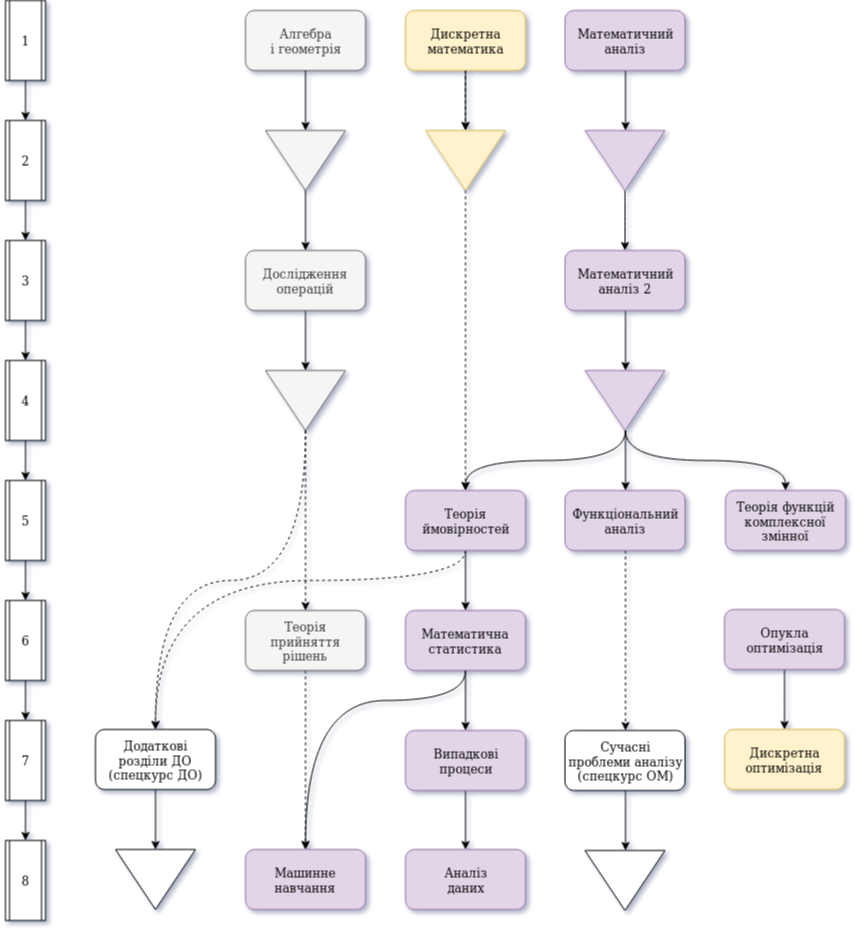
\includegraphics[scale=0.57]{CourseworkTree_1.png}
\end{figure}


\begin{figure}[ht]
\centering
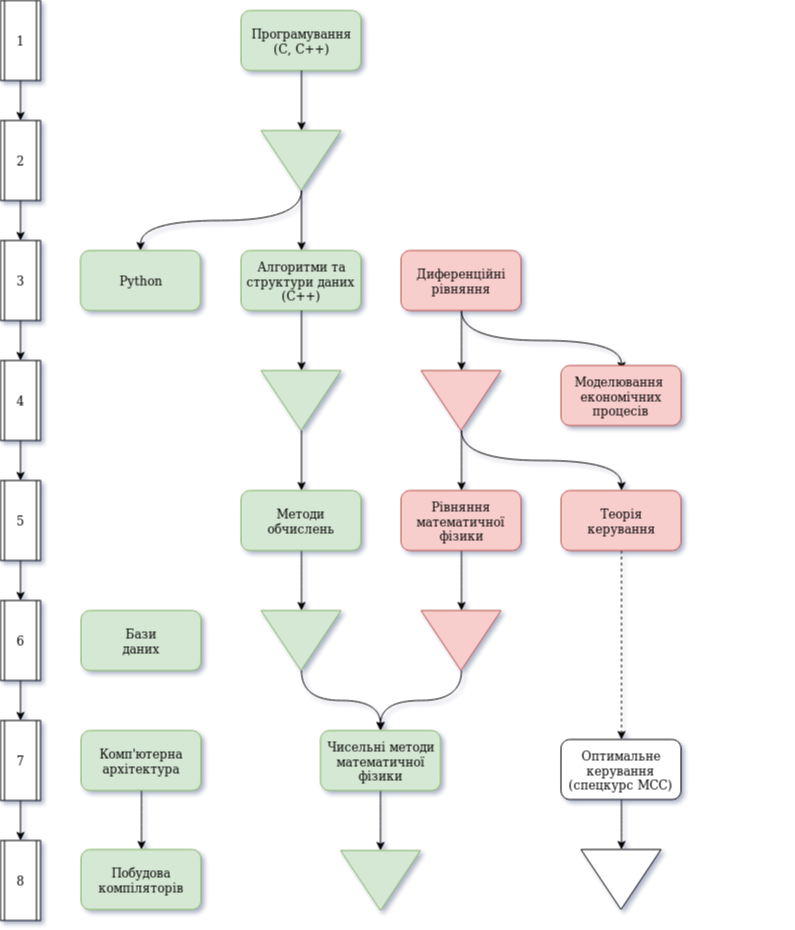
\includegraphics[scale=0.57]{CourseworkTree_2.png}
\end{figure}



\end{document}